\newcommand{\erdatamodaler}{ERwin Data Modeler~}

\chapter{РАЗРАБОТКА ФУНКЦИОНАЛЬНОЙ И \\СТРУКТУРНОЙ СХЕМ УЗЛА}

К разработке предлагается устройство ресинхронизации данных. Определим структурные элементы устройства, принцип и порядок его работы.

\section{Организация взаимодействия с устройством}
Взаимодействие с устройством производится посредством передачи восьмибитного слова на вход wdata. Аппаратный блок осуществляет запись данных во внутреннюю память по сигналам тактового генератора домена источника данных wclk, основываясь на состоянии входных сигналов wrst, wen и служебных сигналов wr\_full,  wptr, rptr.

Чтение из устройства ресинхронизации производится посредством считывания тридцатидвухразрядного слова, генерируемого на выходе rdata. Аппаратный блок осуществляет чтение данных из внутренней памяти по сигналам тактового генератора домена получателя данных, основываясь на состоянии входных сигналов rrst, ren  r\_empty wptr, rptr, rdredy.

\section{Организация памяти}

Устройство хранит данные в собственной памяти. Устройство может одновременно хранить шестнадцать восьмибитных слов, используя для их адресации пятиразрядный адрес, в котором старший бит призван реализовать возможность контроля заполнения и опустошения очереди. 

Возможность асинхронного сброса памяти не реализована в силу того, что обычно память в устройствах, реализуемых на ПЛИС представлена в виде блочной оперативной памяти и выделенной оперативной памяти. Эти ресурсы обычно не поддерживают сброс. Сброс возможно реализовать в регистрах. 



\section{Тактирование}
Управление устройством производится по двух синхросигналам wclk и rclk. С целью оптимальной работы цифрового устройства при передаче данных из одного домена синхросигнала в другой тактовые сигналы входного и выходного каналов сделаны независимыми, однако тактовая частота для выхода очереди составляет как минимум $\dfrac14$ от тактовой частоты входного интерфейса FIFO.

Для корректной передачи и предотвращения потери данных, а также с целью борьбы с метастабильностью в случае независимых тактовых сигналов используются группа синхронизирующих триггеров, которые передают текущее состояние адреса чтения и адреса записи между клоковыми доменами. Основываясь на значениях данных адресов делается вывод о заполненности и пустоте очереди. 

\section{Адресация}

Адресация в памяти реализована с помощью двух пятиразрядных переменных, хранящих адрес ячеек,  с которыми будут произведены операции чтения и записи при следующем синхросигнале.

Важной частью работы устройства является работа с памятью. Необходимо избежать потери и перезаписи не переданных данных. С этой целью на каждом шаге работы схемы осуществляется проверка и сравнивание адресов чтения и записи.

Во время работы схема хранит адреса в виде рефлексивного двоичного кода Грея. Выбор в сторону кода Грея сделан для снижения критичности ошибки определения адреса чтения или записи при его передаче. 

В случае использования кода Грея при переходе к следующему адресу изменяется только один бит, и даже если схема не сможет верно определить значение адреса~---~посчитает, что адреса не изменился, это не приведет к нарушению работы системы. 

В то время как при использовании прямого двоичного кода ошибка синхронизации неизбежна. При переходе могут изменяться все биты адреса (например при переходе $01111 \to 1000$). В данном случае значение адреса является полностью неопределенным. Это может привести к нарушению в работе устройства в целом.

Когда указатели чтения и записи равны, это указывает на то, что FIFO пуст. Эта ситуация возникает во время операции сброса или когда было произведено чтение последнего слова в FIFO, как показано на Рисунке \ref{fig:empty-fifo}.

\begin{figure}[h!]
	\centering
	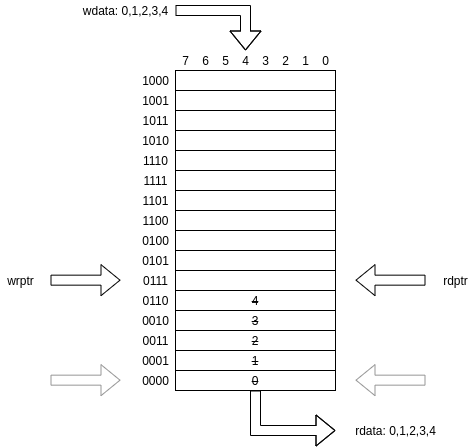
\includegraphics[width=0.7\linewidth]{course-scheme/images/empty-fifo}
	\caption{Все данные прочитаны. Очередь пуста}
	\label{fig:empty-fifo}
\end{figure}

Когда указатели чтения и записи снова равны, это означает, что очередь заполнена и дальнейшая запись не может быть произведена. Эта ситуация возникает, когда переменная адреса записи переполняется, как показано на Рисунке \ref{fig:full-fifo}.

\begin{figure}[h!]
	\centering
	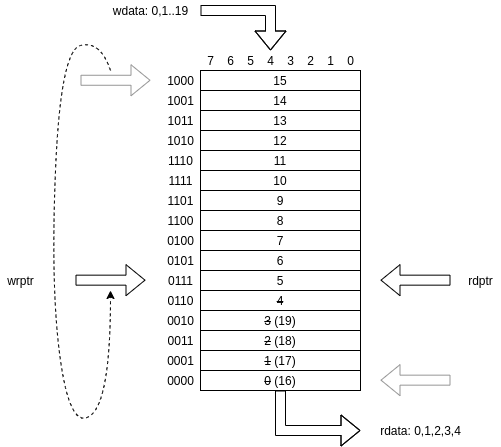
\includegraphics[width=0.7\linewidth]{course-scheme/images/full-fifo}
	\caption{Очередь заполнена. Запись не допустима}
	\label{fig:full-fifo}
\end{figure}

В обоих случаях адреса записи и чтения указывают на одну и ту же ячейку памяти, но при этом ситуации являются противоположными, что усложняет логику определения текущего состояния памяти цифрового устройства.

С целью определения текущего состояния асинхронной очереди необходимо использовать на один бит больше, чем требуется для адресации всех ячеек запоминающего устройства. Сравнение этого бита даст ответ о состоянии памяти в случае, когда указатели чтения и записи окажутся равны.

Пятиразрядные сигналы wr\_full и rd\_empty, позволяющие организовать корректную работу с устройством, формируются с помощью следующих логических условий.
\begin{align}
	 wr\_full = &\left(wptr  == \left\{!rptr[4:3],rptr[aw-2:0]\right\}\right);\\
	 &rd\_empty = \left(wptr  == rptr\right)
\end{align}

В устройстве необходимо реализовать проверку обращения к одному элементу памяти. Чтение по данному адресу должно быть заблокировано до тех пор, пока адрес записи не перестанет указывать на данную ячейку памяти.

При каждом приходящем тактовом сигнале устройство осуществляет сравнение адресов чтения и записи, предварительно производя с ними промежуточные действия. Приведем список преобразований и производимых операций.

\begin{itemize}
	\item перевод из прямого двоичного кода в рефлексивный код Грея;
	\item сохранение текущего значения в регистре;
	\item передача значения адреса в синхронизационные регистры;
	\item перевод из рефлексивного кода Грея в прямой двоичный код;
	\item синхронизация приходящего адреса генератором соседнего домена синхронизации;
	\item сравнение адресов чтения и записи.
\end{itemize}

Данные операции производятся с адресом чтения и записи отдельно. Порядок следования этих операций можно пронаблюдать на Рисунке \ref{fig:signal-process}.

\begin{figure}
	\centering
	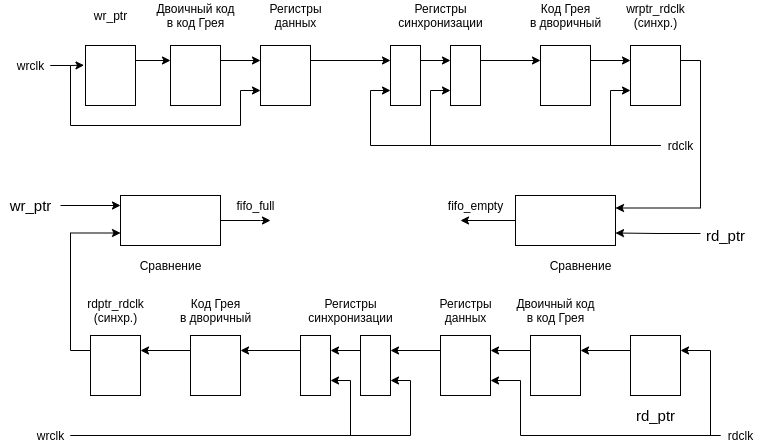
\includegraphics[width=0.7\linewidth]{course-scheme/images/signal-process}
	\caption{Обработка адресов чтения и записи}
	\label{fig:signal-process}
\end{figure}



\section{функциональная схема узла}
Предлагается для построения устройства ресинхронизации данных, работающего в режиме очереди с независимыми тактовыми сигналами, использовать данную функциональную схему (см. Рисунок \ref{fig:unit-design}).

\begin{figure}
	\centering
	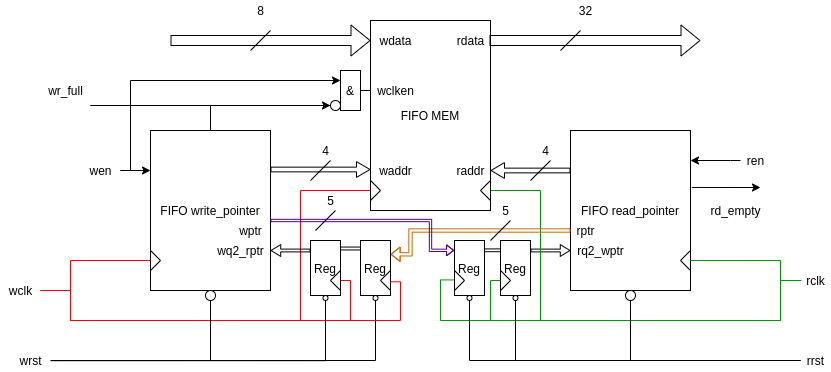
\includegraphics[width=1\linewidth]{course-scheme/images/unit-design}
	\caption{Функциональная схема устройства}
	\label{fig:unit-design}
\end{figure}


Приведем описание входов, выходов и служебных сигналов устройства.


\begin{table}[htbp]
	\caption{}
	\centering
	\fontsize{12}{16pt}\selectfont
	\begin{tabular}{|l|l|}
		\hline
		\multicolumn{1}{|c}{\textbf{Название}} & \multicolumn{1}{|c|}{\textbf{Назначение}} \\ \hline
		asize  &  размер адреса данных с учетом адресации MSB \\ \hline
		dsize  &  размер данных в битах \\ \hline
		mem  &  ячейки памяти очереди \\ \hline
		rbin  &  текущий адрес чтения в бинарном коде \\ \hline
		rbinnext  &  адрес чтения в бинарном коде в следующем такте \\ \hline
		rclk  &  тактирование на чтение данных \\ \hline
		rdata  &  данные на чтение \\ \hline
		rden  &  разрешение на чтение \\ \hline
		rdredy  &  готовность выдать данные \\ \hline
		rempty  &  сигнал пустоты очереди (прочтено все, что записано) \\ \hline
		rempty\_next  &  пустота очереди на следующем такте \\ \hline
		rgray  &  текущий адрес чтения в коде Грея \\ \hline
		rgraynext  &  адрес чтения в коде Грея в следующем такте \\ \hline
		rq1\_wgray  &  адрес чтения в первом синхро-триггере \\ \hline
		rq2\_wgray  &  адрес чтения во втором синхро-триггере \\ \hline
		rrstn  &  сброс указателя чтения \\ \hline
		wbin  &  текущий адрес записи в бинарном коде \\ \hline
		wbinnext  &  адрес записи в бинарном коде в следующем такте \\ \hline
		wclk  &  Тактирование на запись данных \\ \hline
		wdata  &  данные на запись \\ \hline
		wfull  &  сигнал заполнения очереди \\ \hline
		wfull\_next  &  заполненность очереди на следующем такте \\ \hline
		wgray  &  текущий адрес записи в коде Грея \\ \hline
		wgraynext  &  адрес записи в коде Грея в следующем такте \\ \hline
		wq1\_rgray  &  адрес записи в первом синхро-триггере \\ \hline
		wq2\_rgray  &  адрес записи во втором синхро-триггере \\ \hline
		wren  &  разрешение на запись \\ \hline
		wrstn  &  сброc указателя записи \\ \hline
	\end{tabular}
	\label{}
\end{table}





\clearpage